\chapter{The MMSODA Toolbox for MATLAB}
\label{ch:mmsoda}

There are various softwares that implement the Master-Worker paradigm. The most commonly used Master-Worker software is probably MPI\index{Message Passing Interface}\index{MPI}, which stands for \textit{Message Passing Interface}. Most cluster computers have some form of MPI installed. We will use the GNU version of OpenMPI\index{MPI!OpenMPI/GNU}\index{OpenMPI/GNU}, since this is the default MPI package at the LISA cluster computer.

We have developed a parallel MATLAB version of SODA \citep[e.g.][]{vrug-diks-gupt-bout-vers-2005} that makes use of MPI. The software package is called `The MMSODA Toolbox for MATLAB', or MMSODA for short (MMSODA stands for MATLAB-MPI-SODA). In this chapter, we will look at how to set it up.

MMSODA merges a number of previously separate softwares, namely SCEM-UA \citep{vrug-gupt-bout-soro-2003}, MOSCEM-UA \citep{vrug-gupt-bast-bout-soro-2003}, SODA \citep{vrug-diks-gupt-bout-vers-2005}, MOSODA \citep{}, pSCEM-UA \citep{}, and pSODA \citep{}. In short, those acronyms imply that: MMSODA can do parameter tuning with or without intermediate state updating by an ensemble Kalman Filter; that MMSODA supports both single-objective and multi-objective optimization; and that the optimization can be run either in series, or in parallel.

The serial/parallel capability is particularly attractive, since it allows the users to set up their optimizations locally on their own machines, thus ensuring a familiar development environment. When the user finishes setting up the optimization, running it on a cluster computer is simply a matter of copying the relevant directory to the cluster storage using standard tools (e.g. WinSCP) and compiling the software by executing a script that comes with the software. Furthermore, MMSODA is fully documented with HTML documentation which can be accessed in the same way as MATLAB's built-in commands, namely through the \texttt{doc} command.

%scemua-so-seq  SCEM-UA
%scemua-so-par  parallel SCEM-UA
%scemua-mo-seq MOSCEM-UA
%scemua-mo-par parallel MOSCEM-UA
%soda-so-seq  SODA
%soda-so-par  parallel SODA
%soda-mo-seq   MO SODA
%soda-mo-par  parallel MO SODA


The remainder of this chapter explains how to set up increasingly sophisticated optimizations within the MMSODA framework. Let's start off with a single-objective SCEM-UA optimization of a benchmark function \texttt{calcLikelihood()}, and let's not do anything in parallel just yet.

\section{MMSODA in `bypass' mode; offline}

\smallq{First download \texttt{esibayes.zip} from $<$somewhere$>$ and\index{todo} unzip into a local directory.}

As you can see, the zip contains a number of directories. Among these, the `mmsoda-toolbox' directory is probably the most important: it contains the matlab toolbox that this chapter is about. Most of the other directories have names like `soda-so-something' or `bypass-mo-something'. The specific meaning of these names will become clear later; for now, it suffices to say that they are example projects of how to use the MMSODA toolbox for MATLAB with different models and different configurations. Finally there are two more directories, one labeled `template-project', and one labeled `other'. The former contains a rudimentary structure of an MMSODA project, whereas the latter contains some files that we will be using later on.

\smallq{Let's get started by making a new directory next to the \texttt{mmsoda-toolbox} directory. Let's call this directory \texttt{example1}. Change directory into \texttt{example1}, and create three directories in it called \texttt{data}, \texttt{model}, and \texttt{results}. (We won't always use all three directories, but MMSODA expects all three to be present regardless of whether they are used). So now you have a directory somewhere on your local storage device that has at least the following subdirectories:
\begin{itemize}
\item{\texttt{./example1}}
\item{\texttt{./example1/data}}
\item{\texttt{./example1/model}}
\item{\texttt{./example1/results}}
\item{\texttt{./mmsoda-toolbox} (which includes a bunch of subdirectories and subsubdirectories that are not relevant for the moment).}
\end{itemize}
}

\smallq{Open MATLAB and set your working directory to \texttt{example1}.}

\smallq{Before we can use the functionality provided by the MMSODA Toolbox for MATLAB, we need to tell MATLAB about its existence by adding the main directory to the MATLAB search path. You must do this using the \texttt{addpath} command as follows:\\
\texttt{>> addpath(\squote{s})}, in which \texttt{s} indicates the location of the MMSODA directory. For example, it could be:\\
\texttt{>> addpath(\squote{C:\textbackslash{}Users\textbackslash{}jspaaks\textbackslash{}esibayes\textbackslash{}mmsoda-toolbox})}\\ on a Windows machine or \\
\texttt{>> addpath(\squote{/home/jspaaks/esibayes/mmsoda-toolbox})}\\
on Linux.
}
\smallq{At the MATLAB prompt, type:\\
\texttt{>> mmsoda --docinstall}\\
to complete the MMSODA setup. In principle, you only have to run this command once per MATLAB session, as long as you do not change the location of MMSODA's main directory on your storage.}

\smallq{Test whether everything works as it should by typing: \\
\texttt{>> doc mmsoda} \\
at the MATLAB command prompt. This should bring up MATLAB's help browser. Click on the link `View HTML documentation for this function in the help browser'. You should now see an overview of the functions comprising the MMSODA Toolbox for MATLAB.}

\smallq{Spend at least 12 minutes to browse through the documentation. In any case, make sure to read the documentation on `mmsoda.m'.}

The function that we want to optimize implements the double-normal probability distribution:
\begin{equation}\label{eq:double-normal}
\begin{align}
p=\frac{1}{2}\cdot{}\frac{1}{\sqrt{2\cdot{}\pi\cdot{}\sigma{}_1}}\cdot{}\mathrm{exp}\left[-\frac{1}{2}\cdot{}\left(\frac{x-\mu_1}{\sigma_1} \right)^2 \right] \quad & + \\
\frac{1}{2}\cdot{}\frac{1}{\sqrt{2\cdot{}\pi\cdot{}\sigma{}_2}}\cdot{}\mathrm{exp}\left[-\frac{1}{2}\cdot{}\left(\frac{x-\mu_2}{\sigma_2} \right)^2 \right] \quad & \\
\end{align}
\end{equation}
with $\mu_1 = -10$, $\sigma_1 = 3$, $\mu_2 = 5$, $\sigma_2 = 1$, respectively. The parameter that is optimized (or, equivalently, whose probability distribution we will estimate by means of the MMSODA Toolbox for MATLAB) is $x$. For example, for $x=4.5$, $p = 0.1760$.

Because MMSODA expects the objective function to return a log-likelihood $l$, we must actually take the natural logarithm of $p$ as the objective score:
\begin{equation}\label{eq:log-likelihood}
l=\mathrm{log}\left(p\right)
\end{equation}

\subsection{Creating the `constants.mat' and `conf.mat' files}

Before we actually start writing any code for this objective function however, let's first create the `conf.mat' and `constants.mat' files that are always needed for running \texttt{mmsoda()}.

\smallq{Start a new text file in the MATLAB editor and save it as `makeconf.m' in the current working directory.}

\smallq{At the first line in `makeconf.m', add the following:\\
\texttt{function makeconf()}\\}

Now we need to edit the contents of `makeconf.m' as follows.

\smallq{At the MATLAB prompt, type \\
\texttt{doc mmsoda} \\
and bring up the HTML documentation for the \texttt{mmsoda()} function.}

Near the bottom of the documentation, there is an overview of the configuration variables that must be specified for a given type of optimization. For our double-normal example, we will use MMSODA in \squote{bypass} mode. This mode is used when the log-likelihood can be estimated directly from the parameter vector, without the need to run a (dynamic) model structure.

\smallq{If you look in the table with the configuration variables, you'll see that only 5 variables are required for running MMSODA in \squote{bypass} mode. These are \texttt{modeStr}, \texttt{objCallStr}, \texttt{parNames}, \texttt{parSpaceHiBound}, and \texttt{parSpaceLoBound}. Make sure you understand the description for each of these.}

\smallq{Return to `makeconf.m' and add the following:\\
\texttt{modeStr = \squote{bypass};}\\
\texttt{objCallStr = \squote{calcLikelihood};}\\
\texttt{parNames = \{\squote{x}\};}\\
\texttt{parSpaceHiBound = [10];}\\
\texttt{parSpaceLoBound = [-30];}\\
}

With the above settings we specify that we want MMSODA to do a bypass run, in which the function `calcLikelihood.m' (which we will create shortly) is optimized. \texttt{calcLikelihood} has one tunable parameter, \texttt{x}. The bounds that we set on the search for the optimal value of \texttt{x} are \texttt{[-30,10]}.

\smallq{At the last line in `makeconf.m', add the following:\\
\texttt{save(\squote{./results/conf.mat})}\\}

\smallq{Save and close `makeconf.m'.}

Next, we need to create `constants.mat' by a similar procedure.

\smallq{Create a new m-file in the current working directory called `makeconstants.m'.}

\smallq{At the first line in `makeconstants.m', type:\\
\texttt{function makeconstants()}}

Now we need to assign the constants, i.e.\,the variables that \texttt{calcLikelihood} needs in order to calculate the log-likelihood according to equations~\ref{eq:double-normal}--\ref{eq:log-likelihood}.

\smallq{In `makeconstants.m' add:\\
\texttt{parMu1 = -10;}\\
\texttt{parSigma1 = 3;}\\
\texttt{parMu2 = 5;}\\
\texttt{parSigma2 = 1;}\\
i.e. the two means and two standard deviations for the double normal distribution.
}

\smallq{At the last line in `makeconstants.m', add\\
\texttt{save(\squote{./data/constants.mat})}
}

\smallq{Save and close `makeconstants.m'.}

Finally, we need to create the objective function m-file that implements equations~\ref{eq:double-normal} and \ref{eq:log-likelihood}.

\subsection{Creating the objective function m-file}

\smallq{Create a new m-file, called `calcLikelihood.m' and save it in the subdirectory `./model'.}

\smallq{Open `./model/calcLikelihood.m'. MMSODA uses a standardized way of passing the input and output arguments to and from the objective function, so the first line is always exactly the same (with the exception of the name of the function \texttt{calcLikelihood}, which may vary), like so:\\
\texttt{function objScore = calcLikelihood(conf,constants,modelOutput,parVec)}
}

\smallq{As a second line, type: \\
\texttt{mmsodaUnpack()}\\
This function uses the information from the input arguments to construct the variable \texttt{x} and assigns it a value based on the value of \texttt{parVec}. Similarly, it uses information from the \texttt{constants} variable to constructs the model constants and to assign them the correct values.}

Now that we have \texttt{parMu1}, \texttt{parSigma1}, \texttt{parMu2}, \texttt{parSigma2}, and \texttt{x} we can calculate the probability density \texttt{dens} as follows:
\begin{verbatim}
dens = (1/(sqrt(2*pi*parSigma1^2))*exp(-(1/2)*((x-parMu1)/parSigma1)^2) + ...
        1/(sqrt(2*pi*parSigma2^2))*exp(-(1/2)*((x-parMu2)/parSigma2)^2))/2;
\end{verbatim}

\smallq{Add this calculation to your \texttt{calcLikelihood} function.}

\smallq{Don't forget that MMSODA expects a log-likelihood however, so as a final line in \texttt{calcLikelihood}, add:\\
\texttt{objScore = log(dens);}}

\smallq{Save and close `calcLikelihood.m'.}

\subsection{Running the optimization locally}

\smallq{Make sure that the current working directory is the `example1' directory. At the MATLAB command prompt, type:\\
\texttt{>> makeconf()}\\
and check that a new file `conf.mat' is created in subdirectory `./results'.}

\smallq{At the MATLAB command prompt, type:\\
\texttt{>> makeconstants()}\\
and check that a new file `constants.mat' is created in subdirectory `./data'.}

\smallq{At the command prompt, type \texttt{clear} to clear the workspace if there are any variables in it.}

\smallq{Now, we are ready to run the optimization. At the MATLAB command prompt, type:\\
\texttt{>> [evalResults,critGelRub,sequences,metropolisRejects,conf] = mmsoda();}\\
and wait for the optimization to finish. Input arguments to \texttt{mmsoda} are not required, since \texttt{mmsoda} knows to look in `./results/conf.mat' for the configuration, in `./data/constants.mat' for the model constants, and in `./model' for the model functions and objective functions.}

%make sure your working directory is bypass-so-test
%in the command window type makeconf
%in the command window type makeconstants
%in the command window type [evalResults,critGelRub,sequences,metropolisRejects,conf] = soda();

Once the optimization finishes, you should have 5 variables in your workspace: \texttt{evalResults}, \texttt{critGelRub}, \texttt{sequences}, \texttt{metropolisRejects}, \texttt{conf}. Refer to the \texttt{mmsoda()} documentation for a description of what these variables are and how they are laid out.

Let's explore the results by making a histogram of the occurence of certain parameter values. You could simply use MATLAB's built-in \texttt{hist} to do this, like so:\\
\texttt{ >> a = -99;}
\texttt{ >> b = size(evalResults,1);}\\
\texttt{ >> hist(evalResults(b+(a:0),conf.parCols(1)))}\\
\texttt{ >> xlabel(\squote{value of parameter R})}\\
\texttt{ >> ylabel(\squote{count})}\\
to visualize the last 100 draws from the parameter space as a histogram.

% use mmsodaMargHist

%\smallq{A tailored }


\smallq{\textit{some exercises with interpretation of the results.}\index{todo}}

\smallq{Refer back to the documentation on the \texttt{mmsoda} function; specifically, browse through some of the configuration options for running MMSODA in `bypass' mode. Alter your `makeconf.m' with the options that you find useful, and re-run the optimization.}

\smallq{When you are satisfied with the way you set up MMSODA locally, you can make preparations for running it in parallel on the LISA cluster computer. Running on LISA requires a so-called `Makefile'\index{Makefile} as well as a jobscript\index{jobscript}, both of which are tricky to write yourself. Therefore, the MMSODA Toolbox for MATLAB comes with a function that helps you generate the correct files by asking a series of questions. At the MATLAB prompt, type:\\
\texttt{>> mmsodaPrepParallelFiles()}\\
and use the following information to answer the questions:\\
\begin{enumerate}\label{li:answers-mmsodaPrepParallelFiles}
\item{the optimization will run on one of the login nodes;}
\item{we want not much verbal feedback from the program;}
\item{we want the default value for MPI\_BUFFER\_SIZE;}
\item{we don't want to use all the cores on the login node;}
\item{we want to start 8 processes;}
\item{we don't want to save the timing information.}
\end{enumerate}\\
(Note that \texttt{mmsodaPrepParallelFiles()} indicates the default answer with brackets, and that you can accept the default by simply pressing Enter.)
}

When \texttt{mmsodaPrepParallelFiles()} finishes, it prints a message in the command window that tells you what file it has just created. This file should be located in the current working directory. We will use it shortly to start the optimization on the cluster. You can take a look a its contents in Notepad or a similar program, but make sure not to change anything. Besides the jobscript, there should also be a new file called `Makefile'. Just like the jobscript, this is also a plain text file, so you can view its contents in Notepad as well. Again, make sure not to accidentally change anything.


\section{MMSODA in `bypass' mode; online}

\smallq{Use WinSCP or the alternative program of your choice to copy the `example1' and `mmsoda' directories, including all of their contents, to your storage on the cluster.}

When you are satisfied with the way you set up MMSODA locally, you can run it on the LISA cluster computer. In order to do so, we must first compile the software into a so-called `binary'\index{binary} or `executable'\index{executable}. You do not need to worry about how this works in detail, it is just a matter of running the Linux \texttt{make} command. \texttt{make} looks for a file called `Makefile' that was just created by \texttt{mmsodaPrepParallelFiles()}. Based on the contents of `Makefile', \texttt{make} collects all the relevant software (your model files, your objective functions, as well as the code that enables communication between the Master and the Workers) and creates two files that are necessary to run your code within MMSODA using multiple cores.

\section{Compiling MMSODA and your model code into a binary}

\smallq{Use PuTTY to start an SSH connection to the LISA cluster.}

\smallq{In the PuTTY terminal, load the MATLAB program and MPI programs by typing:\\
\texttt{module load matlab}\\
This command will not give any feedback on the success or otherwise of the command, but you could check by typing the following command:\\
\texttt{module list}\\
which should now include MATLAB. Next, type\\
\texttt{module load openmpi/gnu}\\
to load the MPI software.
}

\smallq{Use the \texttt{cd} command to set `example1' as your current directory.}

\smallq{Now we are ready to compile. At the terminal, type:\index{Linux commands!make@\texttt{make}}\\
\texttt{make}\\
You should see some text scrolling over your screen---it takes a while to complete. The \texttt{make} command looks for a file called `Makefile'\index{Makefile} in the current directory, and uses the information in it to correctly build the binary `matlabprog' and the library that it needs, called `libmmpi.so'.}

\smallq{After \texttt{make} finishes, list the directory contents with \texttt{ls -l} and verify that
you now have two extra files `matlabprog' and `libmmpi.so'.}

Starting the optimization requires that we adjust the `permission bits'\index{permission bits} for the `run-mmsoda.sh' file we just created on your local machine. Permission bits indicate what a specific user is allowed to do with a particular file. (You may know the same concept from Windows, where you can sometimes have `Read-only' versions of a file). The permission bits are listed as the first 10 columns in the output from \texttt{ls -l}:
\needspace{12em}
\begin{lstlisting}[style=basic,style=bash]
jspaaks@login1:~/esibayes/example1$ ls -l
total 204
drwxr-xr-x 2 jspaaks jspaaks     26 Jan 16 16:09 data
-rwxrwxr-x 1 jspaaks jspaaks 172792 Jan 18 11:57 libmmpi.so
-rw-r--r-- 1 jspaaks jspaaks    176 Jan 16 16:02 makeconf.m
-rw-r--r-- 1 jspaaks jspaaks    120 Jan 16 15:06 makeconstants.m
-rw-rw-r-- 1 jspaaks jspaaks   1357 Jan 16 16:10 Makefile
-rwxrwxr-x 1 jspaaks jspaaks  11969 Jan 18 11:57 matlabprog
drwxr-xr-x 2 jspaaks jspaaks     29 Jan 16 16:09 model
drwxr-xr-x 2 jspaaks jspaaks   4096 Jan 16 17:36 results
-rw-r--r-- 1 jspaaks jspaaks    580 Jan 18 13:26 run-mmsoda.sh
jspaaks@login1:~/esibayes/example1$
\end{lstlisting}
For `run-mmsoda.sh', the permissions are set to \texttt{-rw-r--r--}. The first character \texttt{-} indicates that `run-mmsoda.sh' is a file (as opposed to a \texttt{d} which would indicate a directory). Characters 2, 3 and 4 (\texttt{rw-}) indicate what you, i.e.\,the currently logged-in user, is allowed to do with `run-mmsoda.sh'. Currently, you are allowed to read from (\texttt{r}) and write to (\texttt{w}) `run-mmsoda.sh'. The \texttt{-} character from the fourth column of \texttt{ls -l} indicates that you are currently not allowed to execute `run-mmsoda.sh' as a script.

\smallq{Change the permission bit for `run-mmsoda.sh' by typing at the prompt:\index{Linux commands!chmod@\texttt{chmod}}\\
\texttt{chmod +x run-mmsoda.sh}\\
Check that the permissions have changed to \texttt{-rwxr--r--} (\texttt{x} for `execute').}

\smallq{Now we can start the optimization in parallel on the login node. At the terminal, type:\\
\texttt{./run-mmsoda.sh}\\
(Don't omit the \texttt{./} at the beginning, otherwise it won't work.)
}

\smallq{\textit{Parallel execution is actually slower than in series due to Amdahl's Law and due to the presence of other users on the login nodes.}\index{todo}}

% % % % % % % % % % % % % % % % % % % % % % % % % % % % % % % % % %

\section{MMSODA in `scemua' mode; offline}

Now that we have a working example of MMSODA in `bypass' mode, let's try our hand at something a little more difficult: optimizing the parameters of a dynamic model. Let's first make a small digression and look at the general structure of dynamic models. Such models simulate the behavior of a number of states over time. As an example, Fig.~\ref{fig:states-and-flows} shows a system in which there are two states. The first state is the water level in a tank which has a small hole in the bottom. The second state is the water level in a tank that has no leaks. The first tank discharges into the second. The rate of discharge $Q$ is dependent on the volume of water in the tank $V_{tank_1}$ and on a resistance parameter $R$ (if there is a big leak in the first tank, the resistance is low, but if the leak is only small, the resistance is high). The model simulates the discharge as follows:
\begin{equation}\label{eq:flow-from-tank1}
Q = \frac{V_{tank_1}}{-R}
\end{equation}

Given the state of the upper tank at a given point in time $V_{tank_1}(t)$, Eq.\,\ref{eq:flow-from-tank1} may be used to calculate the corresponding flow at time $t$. Furthermore, the current state $V_{tank_1}(t)$ and flow $Q(t)$ may be used to simulate the state at a later time, $t+\Delta{}t_{sim}$, provided that $\Delta{}t_{sim}$ is sufficiently small:
\begin{equation}\label{eq:numerical-integration-tank1}
V_{tank_1}(t+\Delta{}t_{sim}) = V_{tank_1}(t) + Q(t)*\Delta{}t_{sim}
\end{equation}

If the initial state of the system $V_{tank_1}(t_0)$ and $V_{tank_2}(t_0)$ is known, and if the resistance parameter $R$ has been assigned, repeated application of Eqs.\,\ref{eq:flow-from-tank1} and \ref{eq:numerical-integration-tank1} thus enables constructing a time series of simulated values for $V_{tank_1}$ and $V_{tank_2}$.

\begin{figure}[htb]
  \centering
    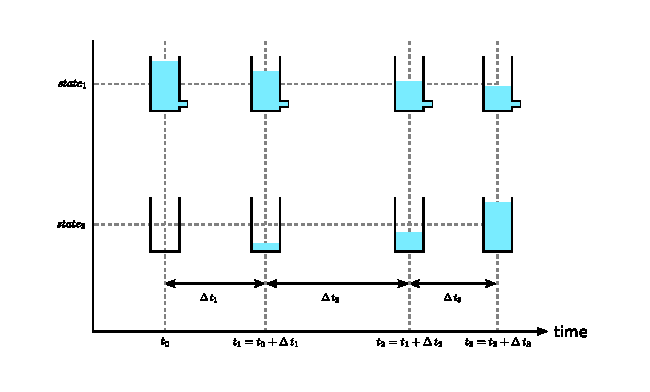
\includegraphics[width=\textwidth]{./../eps/states-and-flows.eps}
  \caption{The general structure of dynamic models.}
  \label{fig:states-and-flows}
\end{figure}

For environmental models, it is very common that not all the parameter values are known beforehand, so it becomes necessary to estimate their values by comparing simulation results to observations of the system's states. The model must therefore be set up such that it returns the system's state at the times for which an observation is available, otherwise the comparison isn't much use. Since the time interval between observations $\Delta{}t_{obs}$ can be (much) larger than the model integration interval $\Delta{}t_{sim}$, multiple model integration steps are often needed in between observation times. Listing~\ref{list:lintank-script} shows a simple MATLAB script that implements the system depicted in Figure~\ref{fig:states-and-flows}.  A copy of the script has been included as `other/lintank\_script.m'.


Over the next few exercises, we will:
\begin{enumerate}
\item{prepare a `constants.mat',}
\item{prepare a `conf.mat',}
\item{prepare the main model m-file by adapting `lintank\_script.m' such that it can be used within the MMSODA framework,}
\item{construct a likelihood function.}
\end{enumerate}
The above four steps are necessary for all types of optimization except `bypass'.


\smallq{Before we start, make sure you understand how the `lintank\_script.m' works by studying Listing~\ref{list:lintank-script} and running through it line-by-line using MATLAB's debugging capabilities.}

\needspace{68em}
\lstinputlisting[style=basic,style=matlab,style=numbered,style=spacious,caption={Simple MATLAB script that implements the system depicted in Figure~\ref{fig:states-and-flows}. A copy of this script has been included as `other/lintank\_script.m'.},label=list:lintank-script]{./../m/lintank_script.m}

\begin{figure}[htb]
  \centering
    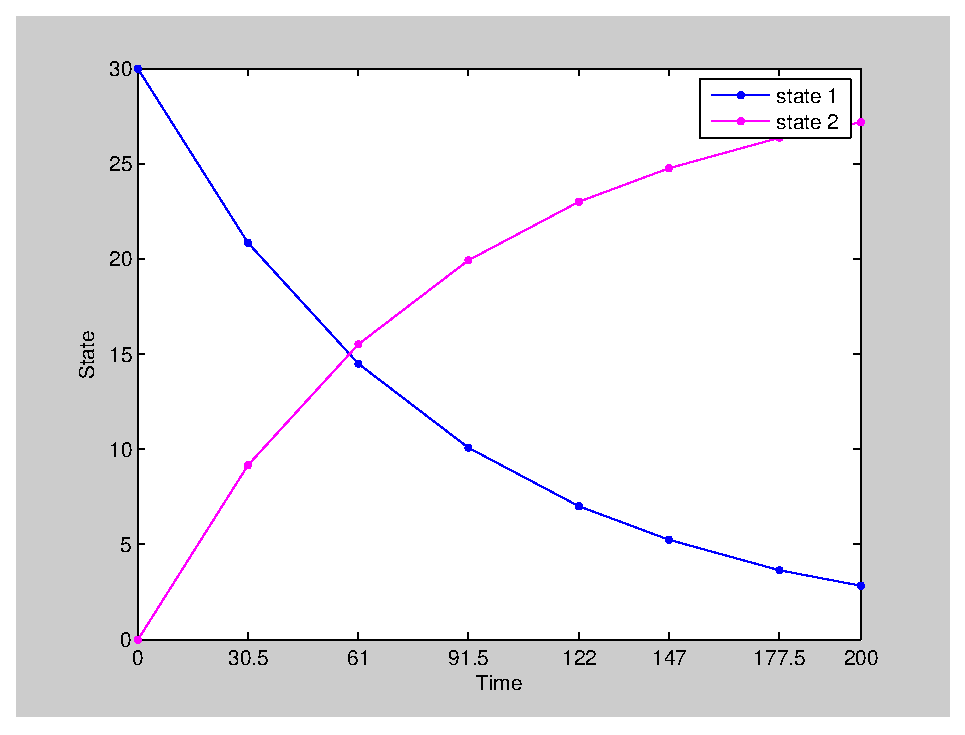
\includegraphics[width=\textwidth]{./../eps/result-of-lintank-script.eps}
  \caption{Result of running the code from Listing~\ref{list:lintank-script}.}
  \label{fig:result-of-lintank-script}
\end{figure}


\smallq{Create a new directory structure with the required subdirectories just like you did before. Verify that the directory is at the same level as the `mmsoda-toolbox' directory.}

\smallq{Read the MMSODA documentation on `the dynamic model' (see Figure~\ref{fig:doc-the-dynamic-model}).}

\begin{figure}[htb]
  \centering
    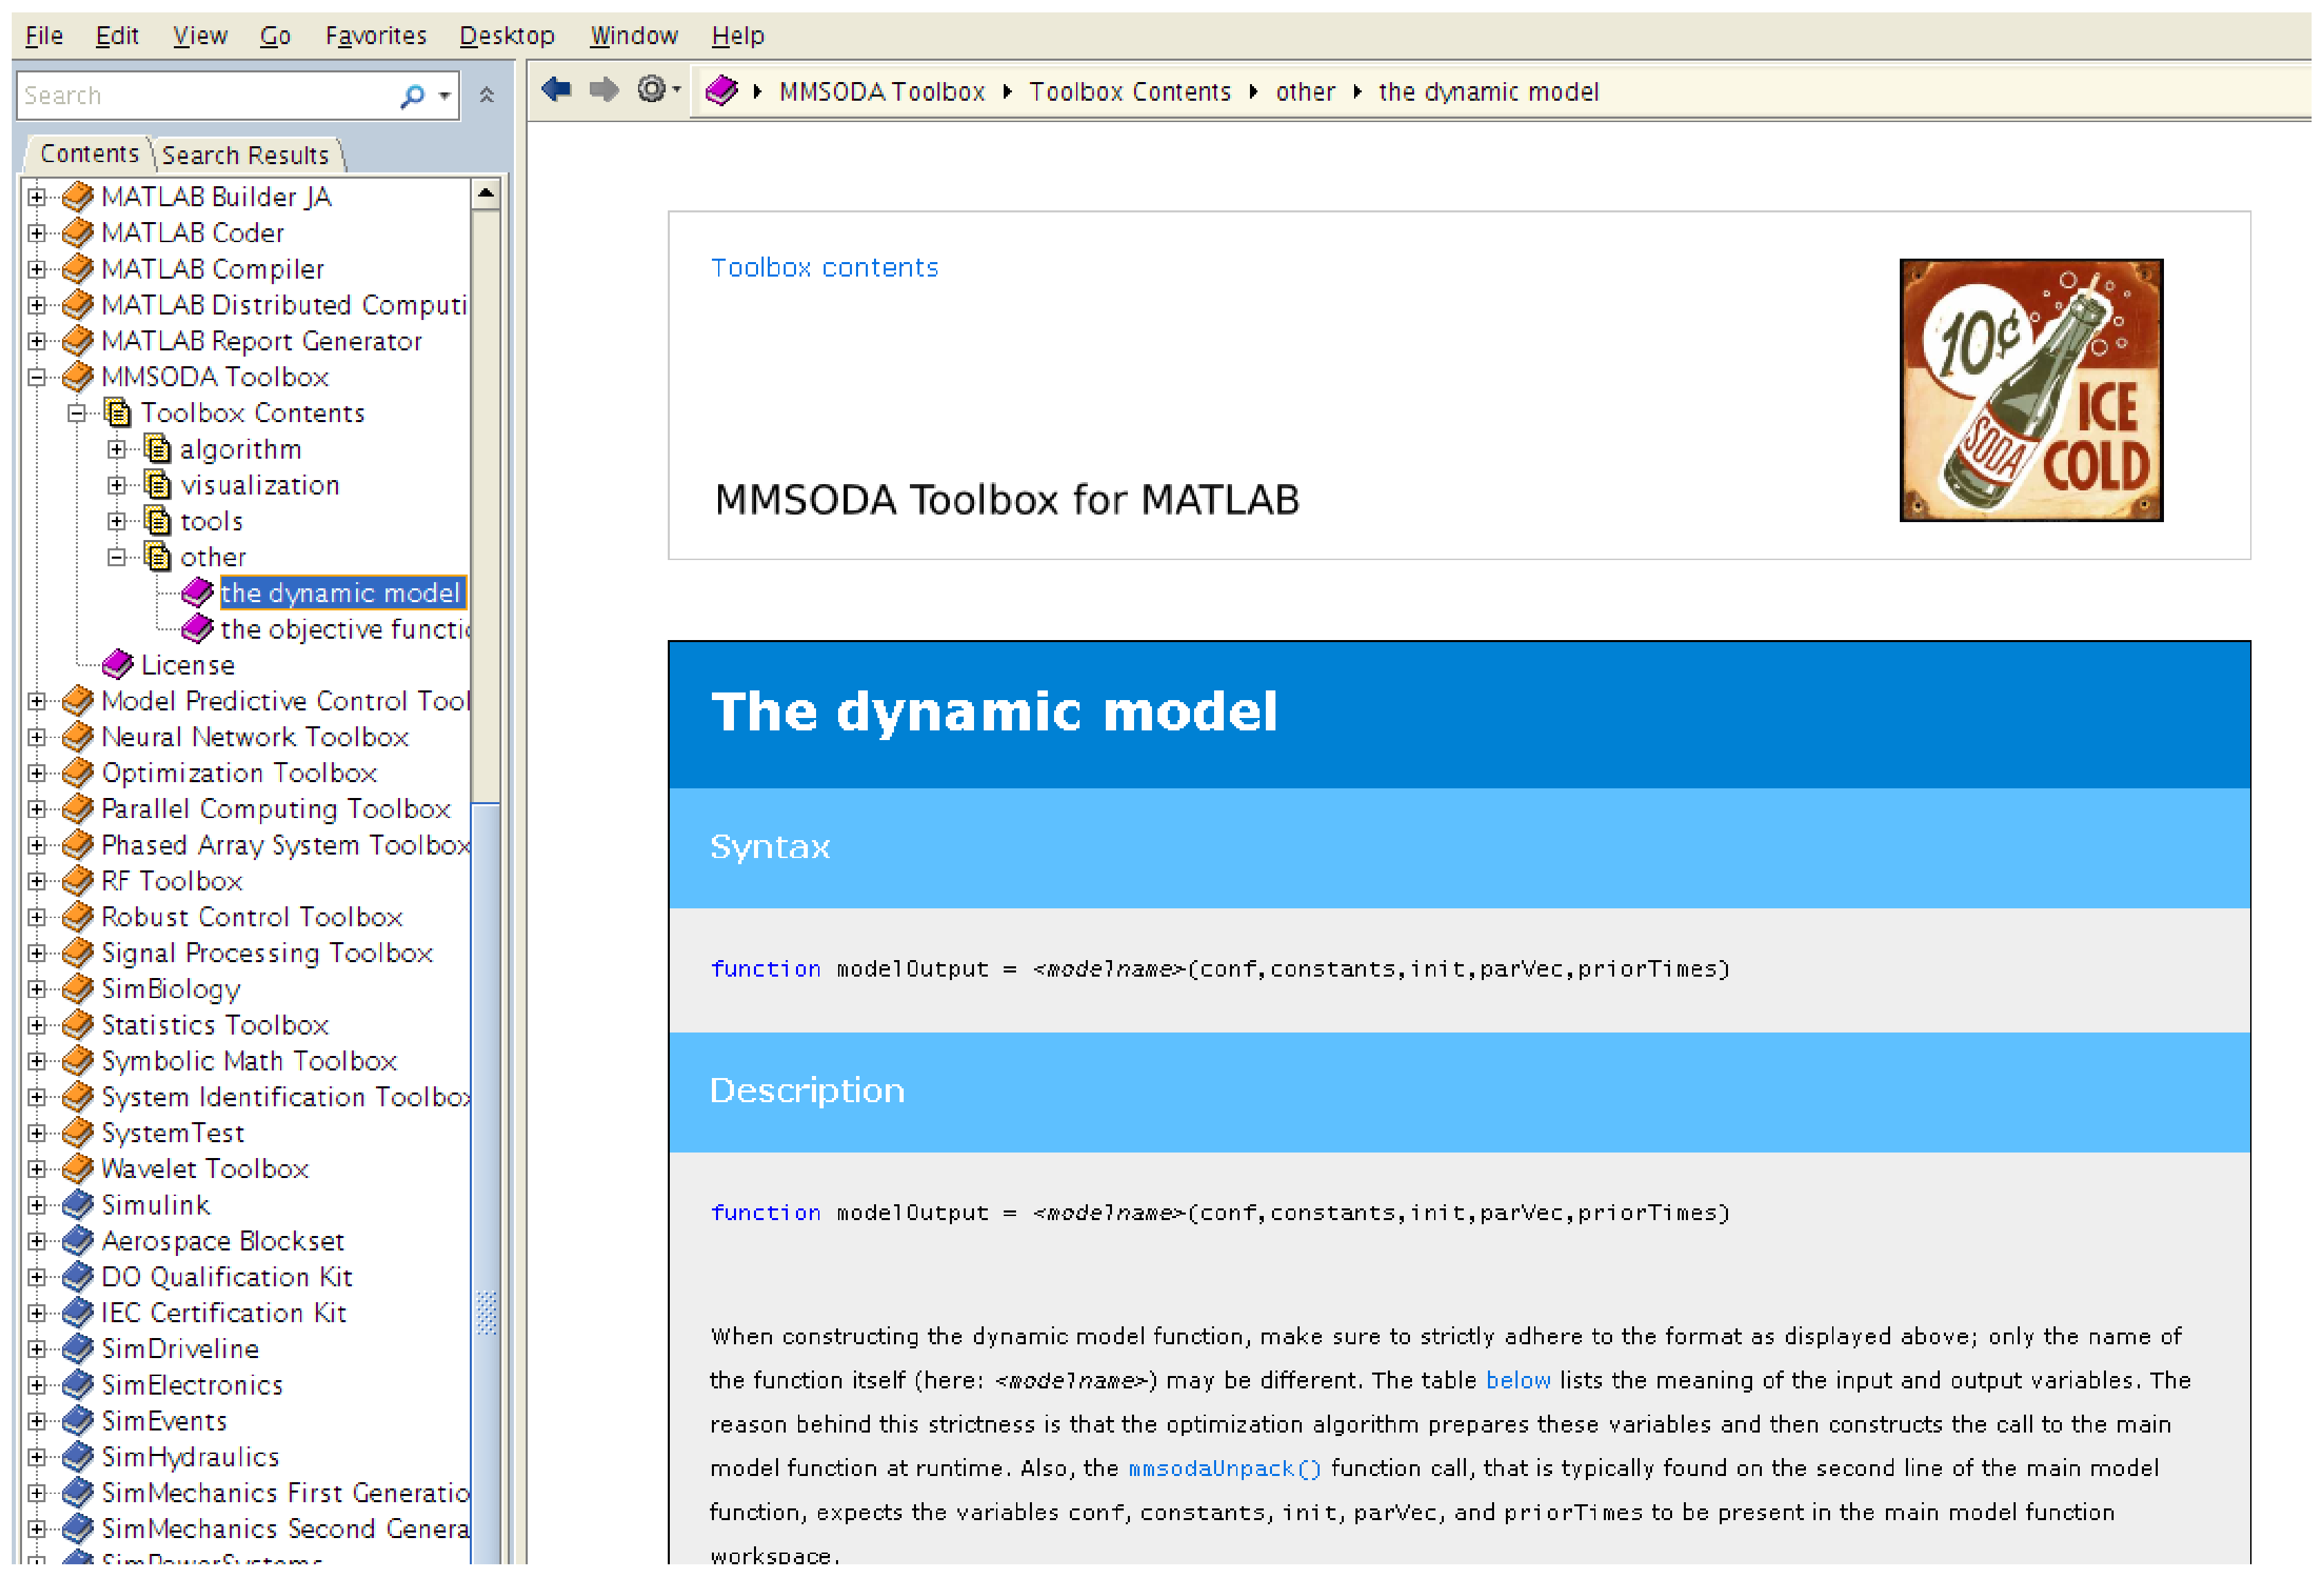
\includegraphics[width=\textwidth]{./../eps/doc-the-dynamic-model.eps}
  \caption{MATLAB documentation on how to set up the dynamic model.}
  \label{fig:doc-the-dynamic-model}
\end{figure}

In the initialization part of Listing~\ref{list:lintank-script}, 10 variables (\texttt{R}, \texttt{state1Init}, \texttt{state2Init}, \texttt{priorTimes}, \texttt{tNow}, \texttt{tEnd}, \texttt{dtSimDefault}, \texttt{rec}, \texttt{state1}, and \texttt{state2}) are created, but only some of these need to included in `constants.mat'. For example, \texttt{R} does not need to be in `constants.mat' because its value will be determined by MMSODA: the variable \texttt{R} is assigned by \texttt{mmsodaUnpack} (which uses the input argument \texttt{parVec} to do so). Similarly, \texttt{priorTimes} and its derivatives \texttt{tNow} and \texttt{tEnd} do not need to be in `constants.mat' because \texttt{priorTimes} is an input argument, too. \texttt{state1}, \texttt{state2}, and \texttt{rec} are all derived from other variables, so they do not need to be part of `constants.mat' either. Essentially, all we need is \texttt{state1Init}, \texttt{state2Init}, and \texttt{dtSimDefault}.

\smallq{Write `makeconstants.m'.}

\smallq{Create a new m-file called `makeconf.m' just like you did before, but this time make sure that the m-file lists the necessary configuration variables for a `scemua' optimization. Refer to the configuration variables table in the MATLAB documentation of \texttt{mmsoda}, and use the information below to set up the optimization:
\begin{enumerate}
\item{Set \texttt{modeStr} to \texttt{\squote{scemua}};}
\item{Set \texttt{modelName} to \texttt{\squote{lintank}}. (We will create `lintank.m' later);}
\item{Set \texttt{objCallStr} to \texttt{\squote{calcLikelihoodState}}. (We will create `calcLikelihoodState.m' later);}
\item{Set \texttt{parNames} to a cell array of strings with the name of the resistance parameter exactly as used in the dynamic part of the model: \texttt{\{\squote{R}\}}. \texttt{R} is the only parameter that will be optimized; }
\item{For the upper boundary of the parameter space, use 1000.0;}
\item{For the lower boundary of the parameter space, use 80.0;}
\item{Fill in the \texttt{priorTimes} values by copying from `lintank\_script.m';}
\item{Set \texttt{nOutputs} to 2.}

\end{enumerate}
} % smallq


\smallq{Copy `lintank\_script.m' to your `model' subdirectory. Rename it to `lintank.m'.}

\smallq{Adapt `lintank.m' to be a function. Refer to the MMSODA documentation on the dynamic model for the proper way of constructing the function's input and output arguments. Remove all lines from the initialization part that are obsolete given that we want to run it within the MMSODA framework. Afterwards, your code should look like that of Listing~\ref{list:lintank-function-1-19}.}

\needspace{20em}
\lstinputlisting[style=basic,style=matlab,style=numbered,style=spacious,caption={First 19 lines of `lintank.m'. You can find a copy of this script at `other/lintank.m'.},label=list:lintank-function-1-19,firstline=1,lastline=19]{./../m/lintank.m}


Next, we need to make sure that we output the correct values. For this, we want to return an array of size \texttt{nOutputs x nPrior}. The $n^{th}$ column in the output argument \texttt{modelOutput} must contain the values pertaining to the $n^{th}$ time in \texttt{priorTimes}. Listing~\ref{list:lintank-function-61-68} shows a simple way of accomplishing this.

\lstinputlisting[style=basic,style=matlab,style=numbered,style=spacious,caption={Last 8 lines of `lintank.m'. You can find a copy of this script at `other/lintank.m'.},label=list:lintank-function-61-68,firstline=61,lastline=68,firstnumber=61]{./../m/lintank.m}



\smallq{Now it's time to test if everything works so far. Make sure MATLAB is in the correct working directory (i.e.\,one level higher than your `data', `model', and `results' directories). At the MATLAB prompt type:\\
\texttt{>> [evalResults,critGelRub,sequences,metropolisRejects,conf] = mmsoda()}\\
and press Enter. If all goes well, MMSODA will start printing various messages to your screen. You should see the message `\texttt{Evaluating parameter sets 1-250}', and if you haven't commented out the visualization part in `lintank.m', you should see 250 plots being made before MMSODA crashes with the following error:}
\begin{lstlisting}[style=basic,style=bash]
Error using eval
Undefined function 'calcLikelihoodState' for input arguments of type 'struct'.
>>
\end{lstlisting}
The error is because MMSODA refers to the configuration variable \texttt{objCallStr}, which you set to \texttt{\squote{calcLikelihoodState}}. When MMSODA attempts to run \texttt{calcLikelihoodState}, this results in an error because we still have to create `calcLikelihoodState.m'.

\smallq{Read the documentation about the objective function (see Figure~\ref{fig:doc-the-objective-function}).}

\begin{figure}[htb]
  \centering
    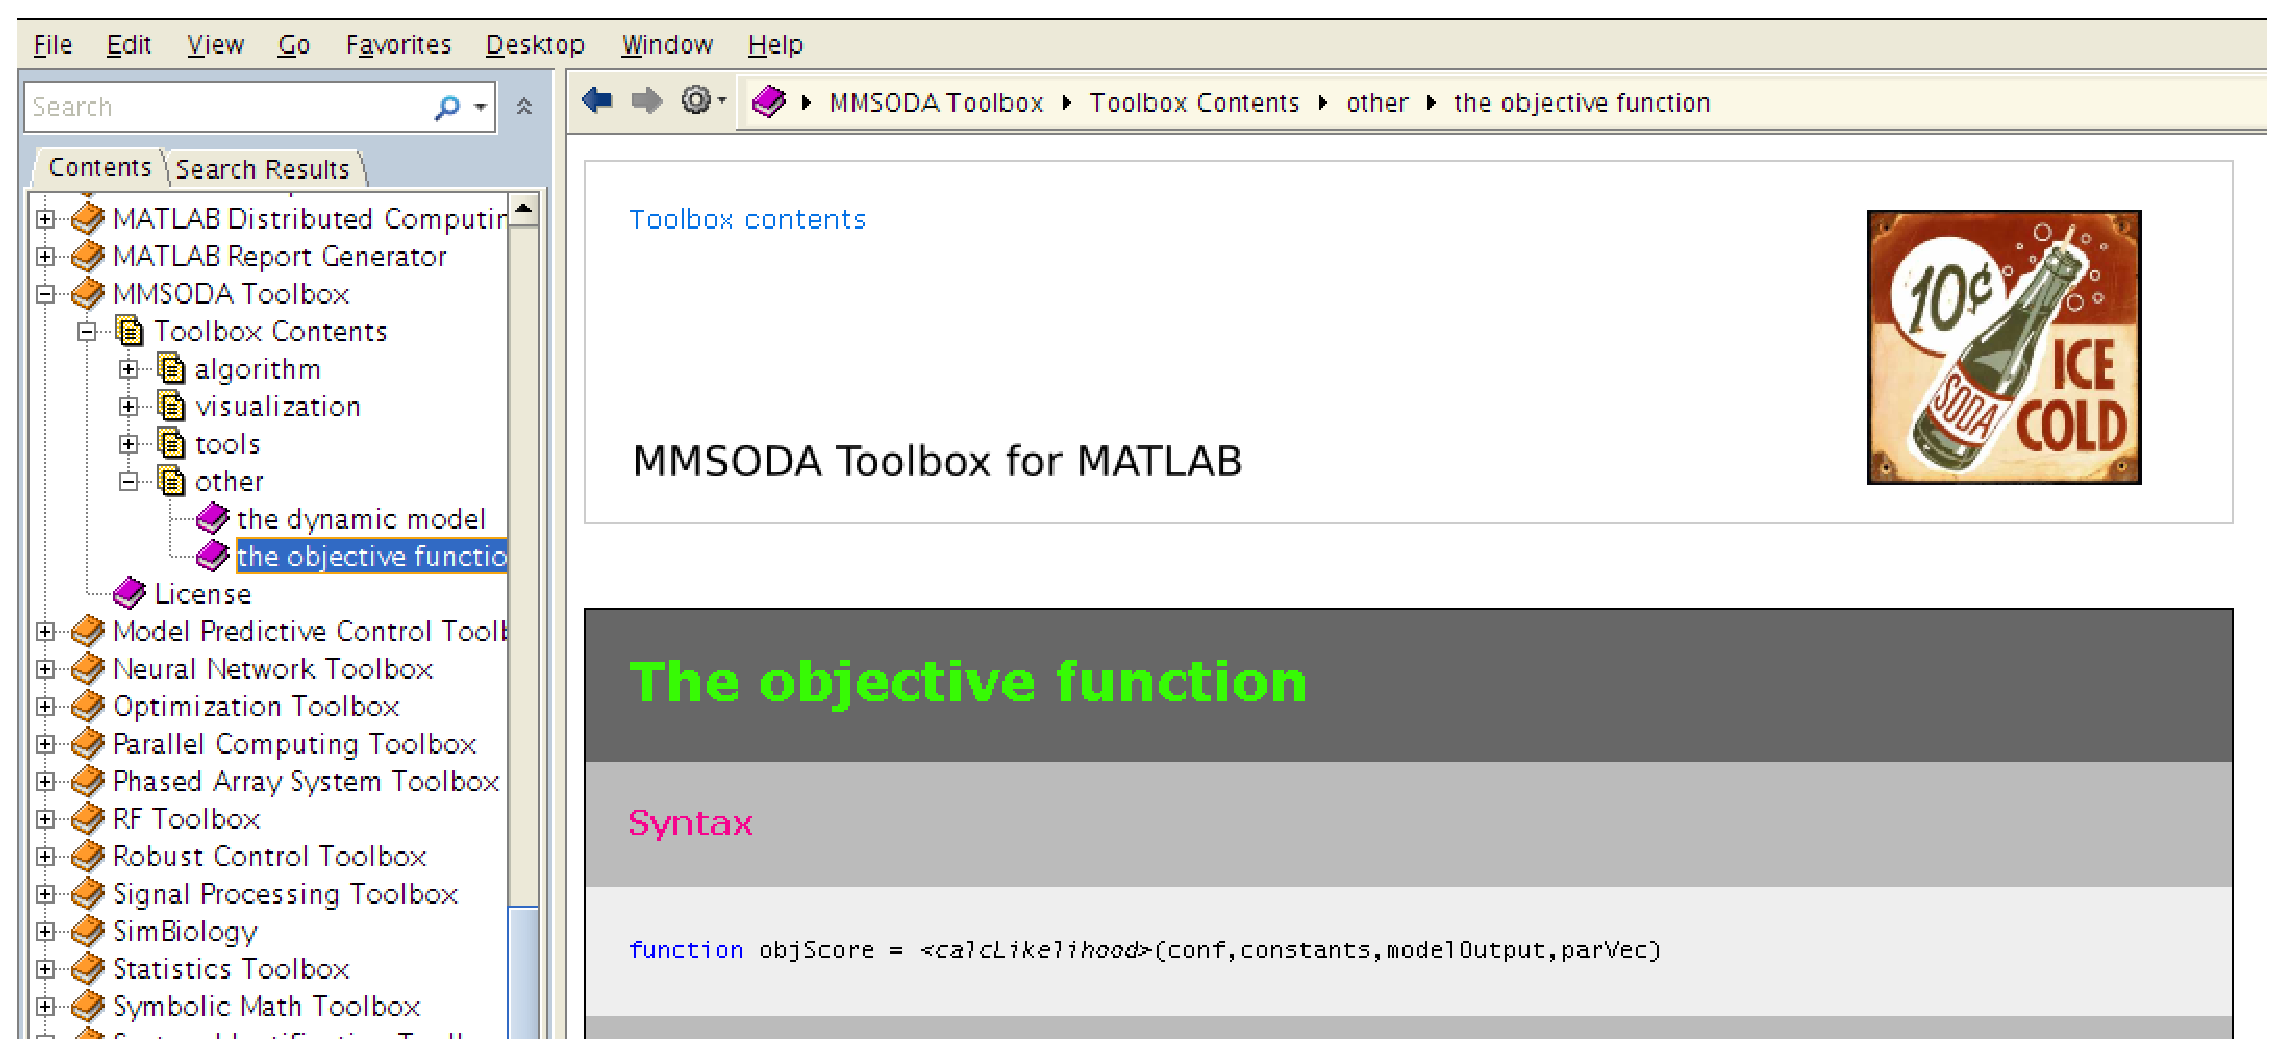
\includegraphics[width=\textwidth]{./../eps/doc-the-objective-function.eps}
  \caption{MATLAB documentation on how to set up the objective function.}
  \label{fig:doc-the-objective-function}
\end{figure}

\smallq{Create a new m-file in the `./model' subdirectory, and call this file `calcLikelihoodState.m'. Refer to the documentation and make sure the first line of the objective function is correct.}

The objective function we will use is related to the sum of squared residuals \index{sum of squared residuals} or SSR\index{SSR}:
\begin{equation}\label{eq:SSR}
\mathrm{SSR} = \displaystyle\sum\limits_{t=1}^{n_o}(\hat{x}_{t}-\tilde{x}_{t})^2
\end{equation}
with $\hat{x}_{t}$ the $t^{\mathrm{th}}$ predicted value of $x$, $\tilde{x}_{t}$ the $t^{\mathrm{th}}$ observed value of $x$, and $n_o$ the total number of observations.

However, we can't use the SSR directly as an objective score, because the SSR is not a log-likelihood (or a probability, for that matter). This problem is easily resolved though, by using the following objective function\footnote{Skip forward to Appendix~\ref{ch:likelihoods-in-optimization} to see how this was derived.\index{todo}}:
\begin{equation}\label{eq:objScore}
\ell = -\frac{1}{2} \cdot{} n_o \cdot{} \mathrm{log}\left(\mathrm{SSR}\right)
\end{equation}

In order to calculate the SSR, we need some observations. These have been prepared already and are located in the `other' directory.

\smallq{Copy `other/lintank-obs.mat' to your `./data' directory.}

\smallq{In `calcLikelihoodState.m', add \\
\texttt{load({\squote{./data/lintank-obs.mat}},\squote{obs},\squote{obsTimes})}
}% smallq


Now that we have the observations in the workspace, we still need to select the corresponding simulations from the \texttt{modelOutput} variable. Refer to the documentation on the objective function for a description. We want to select all values pertaining to the first state (since this is the state that we have observations for). We can do so by:
\needspace{15em}
\begin{lstlisting}[style=basic,style=matlab]
% row of interest in 'modelOutput' is #1
r = 1;
nPriors = 4;
nObs = nPriors-1;

% extract the relevant row from 'modelOutput'
sim = modelOutput(r,1:nPriors);

% Calculate the SSR, but ignore the first entry in 'obs' and 'sim' because those are always
% exactly the same anyway
ssr = sum((obs(1,2:nPriors)-sim(1,2:nPriors)).^2);

% use the SSR to calculate the likelihood
objScore = -(1/2) * nObs * log(ssr);
\end{lstlisting}


\smallq{Add the command lines above to your \texttt{calcLikelihoodState} in order to let it calculate the SSR and the objective score according to Eq.~\ref{eq:objScore}.}

\smallq{Make sure you are still in the right working directory. At the MATLAB prompt, type:\\
\texttt{>> [evalResults,critGelRub,sequences,metropolisRejects,conf] = mmsoda()}\\
}


Currently, \texttt{calcLikelihoodState} loads the observations from file every time it needs to calculate the \texttt{objScore}. Since file operations are much slower than memory operations, it is more efficient to load the observations just once (during creation of the constants), and then keep them in the computer's memory.

\smallq{Cut the \texttt{load} statement from \texttt{calcLikelihoodState} and paste it into `makeconstants.m'. Make sure to re-run \texttt{makeconstants()}, otherwise `./data/constants.mat' will remain unchanged.}

\smallq{Re-read the documentation on MMSODA's \texttt{mmsodaUnpack()} function. Go back to `calcLikelihoodState.m' and use \texttt{mmsodaUnpack()} to make the observations available in the objective function's workspace.}

\smallq{\textit{some interpretation of results}.}

\section{MMSODA in `scemua' mode; online}

\smallq{Generate a `Makefile' and a jobscript using \texttt{mmsodaPrepParallelFiles()}. Use the same answers as those given on page~\pageref{li:answers-mmsodaPrepParallelFiles}. }

\smallq{Copy the working directory to LISA using WinSCP or an alternative program. Make sure the directory is at the same level as the `mmsoda-toolbox' directory that should still be present on the remote system.}

\smallq{Use PuTTY to start an SSH connection to the LISA cluster.}

\smallq{Load the necessary software modules and compile your m-files together with the MMSODA m-files.}

\smallq{Add the executable permission to `run-mmsoda.sh'.}

\smallq{Start the optimization interactively on the login node.}


\section{MMSODA in scemua mode online}
\section{MMSODA in reset mode offline}
\section{MMSODA in reset mode online}
\section{MMSODA in soda mode offline}
\section{MMSODA in soda mode online}
